\section{Auswertung}
\label{sec:Auswertung}

\subsection{Brechungsindizes über die Fresnel Formel bestimmen}
Der gemessene Dunkelstrom ist $I_\text{dunkel} = 1.4 \unit{\nano\ampere}$. Dieser wird bei den folgenden Berechnungen von den gemmesenen Intensität abgezogen.
Die gemessenen Intesitäten für das senkrecht polarisiertem Licht sind in der Tabelle \ref{tab:senk} und 
die für parallel polarisiertem Licht in Tabelle \ref{tab:para} dargestellt.
Zur Berchnung des Brechungsindex für Silizium werden die Formeln \ref{eq:Esenk} und \ref{eq:Epara} verwendet.
Dabei gilt 
\begin{equation*}
  \frac{E_r}{E_e} = \sqrt{\frac{I(\alpha)}{I_0}} = E,
\end{equation*}
da die Intesität des Lichts proportional zum Quadrat der Amplitude des E-Feldes.
Bei beiden Messungen wurde ein Nullstrom von $I_0 = 180 \unit{\micro\ampere}$ gemessen.
Die Formeln \ref{eq:Esenk} und \ref{eq:Epara} werden nach $n$ umsgestellt.
Damit ergibt sich für den Brechungsindex bei senkrecht polarisiertem Licht
\begin{equation}
  n_\parallel = \Bigl(\frac{E+1}{E-1}\Bigr)^2\frac{1}{2 \cos(\alpha)^2}+\sqrt{\frac{1}{4 \cos(\alpha)^2}\Bigl(\frac{E+1}{E-1}\Bigr)^4-\Bigl(\frac{E+1}{E-1}\Bigr)^2 \tan(\alpha)^2}
\end{equation}
und für den Brechungsindex bei senkrecht polarisiertem Licht
\begin{equation}
  n_\perp = \sqrt{\frac{1+ E^2+ 2 E \cos(2 \alpha)}{1- 2 E+ E^2}}.
\end{equation}
Die Ergebnisse der Brechungindexe werden ebenfalls in der Tabelle \ref{tab:senk} und \ref{tab:para} dargestellt.
\begin{table}[H]
  \centering
  \caption{Gemessene Intensitäten und berechneter Brechungsindizes bei senkrecht plarisierten Licht.}
  \label{tab:senk}
  \begin{tabular}{c c c c c c}
    \toprule
    $\alpha /°$ & $I / \unit{\micro\ampere}$ & $n$ & $\alpha /°$ & $I / \unit{\micro\ampere}$ & $n_\perp$\\
    \midrule          
    4  &  54  & 3.41    & 48 &  92   & 4.09   \\
    6  &  60  & 3.71    & 50 &  92   & 3.94   \\ 
    8  &  64  & 3.91    & 52 &  97   & 4.09    \\
    10 &  66  & 4.01    & 54 &  96   & 3.85    \\
    12 &  64  & 3.87    & 56 &  100  & 3.92    \\
    14 &  62  & 3.73    & 58 &  100  & 3.72    \\
    16 &  66  & 3.92    & 60 &  100  & 3.53    \\
    18 &  64  & 3.77    & 62 &  100  & 3.33   \\ 
    20 &  70  & 4.06    & 64 &  100  & 3.13    \\
    22 &  70  & 4.01    & 66 &  110  & 3.44    \\
    24 &  72  & 4.07    & 68 &  110  & 3.19    \\
    26 &  72  & 4.01    & 70 &  115  & 3.20    \\
    28 &  72  & 3.94    & 72 &  120  & 3.20    \\
    30 &  74  & 3.99    & 74 &  130  & 3.52    \\
    32 &  76  & 4.02    & 76 &  135  & 3.50   \\ 
    34 &  78  & 4.06    & 78 &  140  & 3.45   \\
    36 &  78  & 3.96    & 80 &  144  & 3.26   \\
    38 &  82  & 4.10    & 80 &  144  & 2.92   \\
    40 &  84  & 4.11    & 82 &  147  & 1.94   \\
    42 &  86  & 4.12    & 84 &  140  & 1.04   \\
    44 &  88  & 4.12    & 86 &  70   & 4.88 \\ 
    46 &  90  & 4.11    &    &       &        \\                 
    \bottomrule
  \end{tabular}
\end{table}
      
\begin{table}[H]
  \centering
  \caption{Gemessene Intensitäten und berechnete Brechungsindizes bei parallel plarisierten Licht.}
  \label{tab:para}
  \begin{tabular}{c c c c c c}
    \toprule
    $\alpha /°$ & $I / \unit{\micro\ampere}$ & $n$ & $\alpha /°$ & $I / \unit{\micro\ampere}$ & $n_\parallel$\\
    \midrule 
    6  &  50  & 3.35  & 48 &  28   & 3.50 \\ 
    8  &  50  & 22.1  & 50 &  27   & 2.33 \\
    10 &  50  & 3.80  & 52 &  24   & 13.15 \\
    12 &  49  & 3.73  & 54 &  20   & 2.34  \\
    14 &  48  & 22.9  & 56 &  20   & 2.28  \\
    16 &  48  & 3.26  & 58 &  18   & 16.12 \\
    18 &  42  & 4.27  & 60 &  14   & 1.83  \\
    20 &  47  & 7.51  & 62 &  14   & 2.51  \\
    22 &  46  & 3.04  & 64 &  12   & 4.22  \\
    24 &  45  & 7.01  & 66 &  11   & 1.65  \\
    26 &  44  & 4.50  & 68 &  9.6  & 3.51  \\
    28 &  44  & 3.05  & 70 &  8    & 2.27  \\
    30 &  41  & 18.29  & 72 &  8.2  & 1.57  \\
    32 &  41  & 3.34  & 74 &  8.6  & 9.02   \\
    34 &  37  & 3.08  & 76 &  9.6  & 1.84  \\
    36 &  38  & 21.0  & 78 &  10   & 1.80  \\
    38 &  37  & 2.76  & 80 &  12   & 15.33  \\
    40 &  36  & 3.85  & 82 &  21   & 2.12  \\
    42 &  34  & 6.27  & 84 &  30   & 3.41   \\
    44 &  32  & 2.45  & 86 &  50   & 8.36   \\
    46 &  30  & 5.42  &    &       &      \\
    \bottomrule
  \end{tabular}
\end{table}

\noindent Die berechneten Brechungsindizes werden nun gemittelt.
Die Unsicherheiten wurden mithilfe von $uncertenties$ berechnet.
Damit ergibt sich 
\begin{equation*}
  \overline{n}_\perp = 3.65 \pm 0.59
\end{equation*}
und\begin{equation*}
  \overline{n}_\parallel = 6.20 \pm 5.98
\end{equation*}    

\subsection{Brechungsindex über den Brewsterwinkel bestimmen}

Der Brewsterwinkel lässt sich bei parallel polarisiertem Licht bestimmen.
Dabei handelt sich um den Winkel, bei dem das Minimum gemessen wurde.
Der Brewsterwinkel ist somit
\begin{equation*}
  \alpha_p = \qty{70 \pm 1}{°}.
\end{equation*}    
Der brechungsindex wird nun über die Formel \ref{eq:Brewster} berechnet.
Für den Brechungsindex ergibt sich damit 
\begin{equation*}
  n_{\alpha_p} = 2.74 \pm 0.14.
\end{equation*}

\noindent In der Abbildung \ref{fig:plot} sind die Messwerte und die jeweiligen Theoriekurven abgebildet.
Bei den Theoriekurven wurde die Formeln \ref{tab:senk} und \ref{tab:para} verwendet.
Für den jeweiligen Brechungsindex wurde der zuvor berechnete Wert $\overline{n}_\parallel$ und $\overline{n}_\perp$ eingesetzt.

\begin{figure}
  \centering
  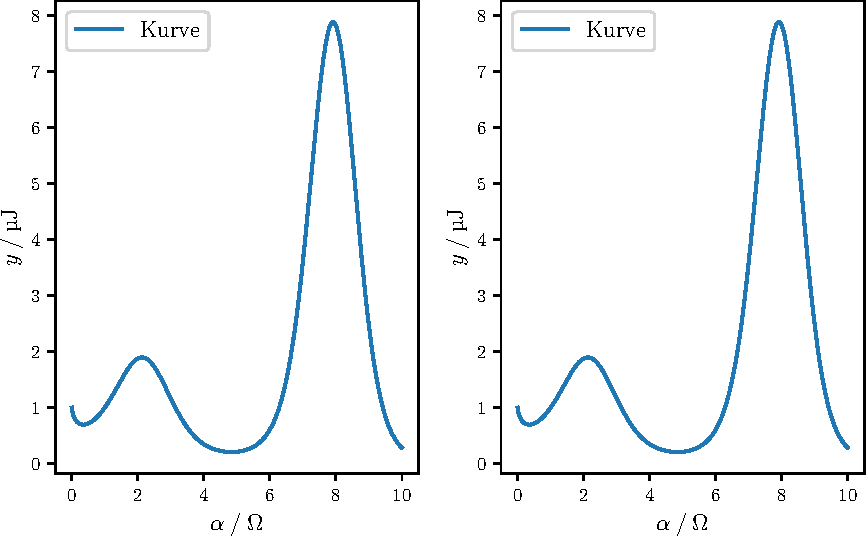
\includegraphics{plot.pdf}
  \caption{Graphische Darstellung der Messwerte und der Theoriekurve.}
  \label{fig:plot}
\end{figure}

